\chapter{Ejercicio 1}

\section{Actividad 1}

\textbf{Actividad 1}. Dada la secuencia de se\~nales {$\phi_{n} (t)=e^{j(n\omega)t}: n \in \mathbb{Z}$}, con $T = \dfrac{2\pi}{\omega}$. Demostrar:

\subsection{A}

\textbf{A)} El per\'iodo fundamental de la se\~nal $\phi_{n}(t)$ es $T_n=\dfrac{2\pi}{n\omega}$. ¿Por qué se puede afirmar que la suma entre \'estas señales está bien definida $\phi_{n}(t)$?

\textbf{i.} Lo primero que realizaremos ser\'a corroborar que $T_n$ es un per\'iodo.

$$\phi_{n}(t+T_n)=\phi_{n}(t)$$

$$e^{jn\omega(t+T_n)}=e^{jn\omega(t)}$$

$$e^{jn\omega(t+\dfrac{2\pi}{n\omega})}=e^{jn\omega(t)}$$

$$e^{jn\omega(t)+jn\omega\dfrac{2\pi}{n\omega}}=e^{jn\omega(t)}$$

$$e^{jn\omega(t)+j2\pi}=e^{jn\omega(t)}$$

$$e^{jn\omega(t)} \cdot e^{j2\pi} = e^{jn\omega(t)}$$

$$e^{jn\omega(t)} \cdot 1 = e^{jn\omega(t)}$$

$$e^{jn\omega(t)} = e^{jn\omega(t)}$$

\textbf{ii.} Para ver que $T_n$ es el per\'iodo fundamental, suponemos que existe un $T'>0$ con $T'<T_n$, tal que $\phi_n(t+T')=\phi_n(t)$

Sabemos que $e^{jn\omega T'} = 1$, por lo que existe un $k \in \mathbb{Z}$ tal que

$$n\omega T'= 2\pi k$$

Despejando $n\omega$

$$T'=\dfrac{2\pi k}{n\omega}$$

Donde si $k=0$ entonces $T'=0$, lo cual contradice lo que postulamos al principio que $T'>0$

Si $|k| \ge 1$, entonces

$$T' \ge \dfrac{2\pi}{|n|\omega} = T_{|n|}$$

Lo cual contradice que $T'<T_n$. Por lo tanto, no existe $T'\in(0,T_n)$ que sea per\'iodo.

\textbf{iii.}

Ahora bien, podemos concluir que la suma $\sum_{n \in \mathbb{Z}} \phi_n(t)$ está bien definida porque todas las señales $\phi_n(t)$ son peri\'odicas con un per\'iodo común $T = \frac{2\pi}{\omega}$ (múltiplo entero de $T_n$). Esto garantiza que la superposición de señales mantenga la periodicidad global.

\vspace{0.5cm}

\subsection{B}

\textbf{B)} Calcular $E_n = (\phi_n(t), \phi_n(t))_T \quad \text{y} \quad (\phi_n(t), \phi_m(t))_T, \quad \forall n,m \in \mathbb{Z}$

Como primer paso definiremos
\[
\langle \phi_n, \phi_m \rangle_T = \frac{1}{T}\int_0^T \phi_n(t)\overline{\phi_m(t)}dt
\]

\textbf{Caso 1: $n = m$}
\begin{align*}
\langle \phi_n, \phi_n \rangle_T &= \frac{1}{T}\int_0^T e^{jn\omega t}e^{-jn\omega t}dt \\
&= \frac{1}{T}\int_0^T 1\,dt = 1 \quad \forall n
\end{align*}

\textbf{Caso 2: $n \neq m$}
\begin{align*}
\langle \phi_n, \phi_m \rangle_T &= \frac{1}{T}\int_0^T e^{j(n-m)\omega t}dt \\
&= \left.\frac{e^{j(n-m)\omega t}}{j(n-m)\omega T}\right|_0^T = 0 \quad \text{(por periodicidad)}
\end{align*}

\vspace{0.5cm}

\subsection{C}

\textbf{C)} La secuencia de señales $\{ \phi_n(t) = e^{j(n\omega)t} : n \in \mathbb{Z} \}$ es base de Fourier.

\textbf{Propiedades requeridas:}
\begin{enumerate}[label=(\roman*)]
\item \textbf{Ortogonalidad}: $\langle \phi_n, \phi_m \rangle_T = \delta_{nm}$ (demostrado en B)
\item \textbf{Completitud}: Cualquier señal $x(t)$ periódica puede expresarse como:
\[
x(t) = \sum_{n=-\infty}^{\infty} C_n \phi_n(t)
\]
\end{enumerate}

\vspace{0.5cm}

\subsection{D}

\textbf{D)} La secuencia de señales $\{ \rho_n^0(t) = \cos(n\omega t) = \tfrac{1}{2}\phi_n(t) + \tfrac{1}{2}\overline{\phi_n(t)} : n \geq 0 \}$ es base de Fourier.

\textbf{Relación con $\phi_n(t)$:}
\[
\cos(n\omega t) = \frac{1}{2}\phi_n(t) + \frac{1}{2}\phi_{-n}(t)
\]

\textbf{Ortogonalidad:}
\[
\langle \rho_n^0, \rho_m^0 \rangle_T = 
\begin{cases}
1 & n = m = 0 \\
\frac{1}{2} & n = m \neq 0 \\
0 & n \neq m
\end{cases}
\]

\vspace{0.5cm}

\subsection{E}

\textbf{E)} La secuencia de señales \[\{ \rho_n^1(t) = \sin(n\omega t) = \tfrac{1}{2j}\phi_n(t) - \tfrac{1}{2j}\overline{\phi_n(t)} : n > 0 \}\] es base de Fourier.

\textbf{Relación con $\phi_n(t)$:}
\[
\sin(n\omega t) = \frac{1}{2j}\phi_n(t) - \frac{1}{2j}\phi_{-n}(t)
\]

\textbf{Ortogonalidad:}
\[
\langle \rho_n^1, \rho_m^1 \rangle_T = 
\begin{cases}
\frac{1}{2} & n = m \\
0 & n \neq m
\end{cases}
\]

\section{Actividad 2}

\textbf{Actividad 2.} Calcular la descomposicion de series $x(t) = \sum_{n \in \mathbb{Z}}$ y $x(t) = a_0 + \sum_{n=1}^{\infty}(a_n \rho_n ^0(t) + b_n \rho_n ^1(t))$ de las siguientes se\~nales. Para luego calcular aproximadamente la energia de la se\~nal usando el teorema de Parseval.

\subsection{Se\~nal sinusoidal rectificada de onda completa}

\begin{figure}[H]
  \centering
  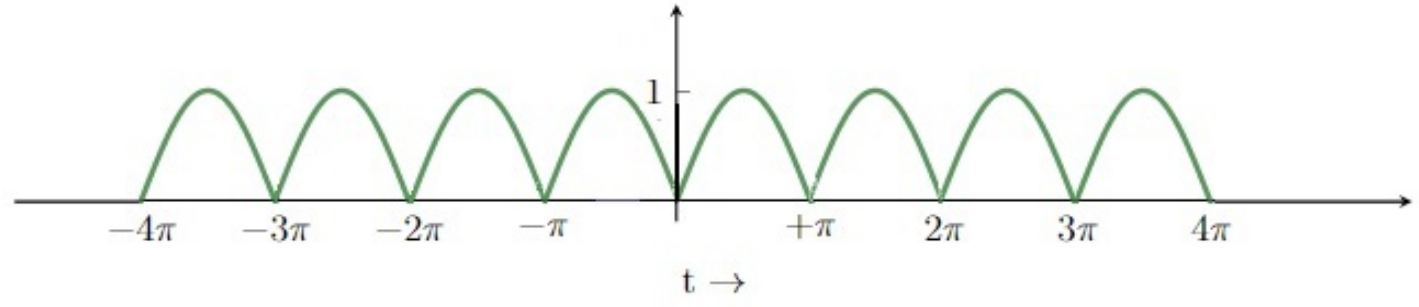
\includegraphics[width=0.8\textwidth]{photos/onda_completa.png}
\end{figure}

La se\~nal se trata de $x(t) = |sen(t)|$.

Primero debemos tomar el per\'iodo de la se\~nal, el cual es igual a $\pi$, para poder calcular el coeficiente $C_n$ el cual esta dado por la siguiente ecuaci\'on.

$$C_n = \dfrac{1}{T} \int_{<T>} x(t) e^{-j(n\omega)t} dt$$

$$C_n = \dfrac{1}{\pi} \int_{0}^{\pi} |sen(t)| e^{-j(n\omega)t} dt$$

Siendo $\omega = \dfrac{2\pi}{T} = 2$

Quedando $e^{-j(n\omega)t} = e^{-j2nt} = cos(2nt)-j\,sen(2nt)$

$$C_n = \dfrac{1}{\pi} \int_{0}^{\pi} |sen(t)| [\cos(2nt) - j sen(2nt)] dt$$

$$C_n = \dfrac{1}{\pi} \bigg[\int_{0}^{\pi} sen(t) cos(2nt) dt + j \int_{0}^{\pi} sen(t) sen(2nt) dt \bigg] $$

Es de importancia saber que $ \int_{0}^{\pi} sen(t) sen(2nt) dt = 0$

$$C_n = \dfrac{1}{\pi} \bigg[\int_{0}^{\pi} sen(t) cos(2nt) dt + 0 \bigg] $$

$$C_n = \dfrac{1}{\pi} \int_{0}^{\pi} \bigg[ \bigg(\dfrac{e^{jt}-e^{-jt}}{j2}\bigg) \cdot \bigg(\dfrac{e^{j2nt}+e^{-j2nt}}{2} \bigg) \bigg] dt $$

En este paso distribuimos

$$C_n = \dfrac{1}{\pi} \int_{0}^{\pi} \bigg[\dfrac{e^{jt(1+2n)}}{j4} + \dfrac{e^{jt(1-2n)}}{j4} - \dfrac{e^{-jt(1-2n)}}{j4} - \dfrac{e^{-jt(1+2n)}}{j4}\bigg] dt $$

Sacamos factor com\'un y ordenamos

$$C_n = \dfrac{1}{\pi} \int_{0}^{\pi} \dfrac{1}{j4} \bigg[e^{jt(1+2n)} - e^{-jt(1+2n)} - e^{-jt(1-2n)} + e^{jt(1-2n)}\bigg] dt $$

$$C_n = \dfrac{1}{j4\pi} \bigg[\dfrac{e^{jt(1+2n)}}{j(1+2n)} \bigg\rvert_{0}^{\pi} - \dfrac{e^{-jt(1+2n)}}{-j(1+2n)} \bigg\rvert_{0}^{\pi} - \dfrac{e^{-jt(1-2n)}}{-j(1-2n)} \bigg\rvert_{0}^{\pi} + \dfrac{e^{jt(1-2n)}}{j(1-2n)} \bigg\rvert_{0}^{\pi} \bigg] $$

$$C_n = \dfrac{1}{j4\pi} \bigg[\dfrac{e^{j\pi(1+2n)}-1}{j(1+2n)} + \dfrac{e^{-j\pi(1+2n)}-1}{j(1+2n)} + \dfrac{e^{-j\pi(1-2n)}-1}{j(1-2n)} + \dfrac{e^{j\pi(1-2n)}-1}{j(1-2n)} \bigg] $$

$$C_n = \dfrac{1}{j4\pi} \bigg[\dfrac{(-1)-1}{j(1+2n)} + \dfrac{(-1)-1}{j(1+2n)} + \dfrac{(-1)-1}{j(1-2n)} + \dfrac{(-1)-1}{j(1-2n)} \bigg] $$

$$C_n = \dfrac{1}{j4\pi} \bigg[\dfrac{-2}{j(1+2n)} + \dfrac{-2}{j(1+2n)} + \dfrac{-2}{j(1-2n)} + \dfrac{-2}{j(1-2n)} \bigg] $$

$$C_n = \dfrac{-2}{j4\pi} \bigg[\dfrac{2}{j(1+2n)} + \dfrac{2}{j(1-2n)} \bigg] $$

$$C_n = \dfrac{1}{2\pi} \bigg[\dfrac{2+2}{(1+2n)(1-2n)}\bigg] $$

$$C_n = \dfrac{1}{2\pi} \bigg[\dfrac{4}{1-4n^2} \bigg] $$

$$C_n = \dfrac{2}{\pi(1-4n^2)} $$

Ahora con el coeficiente podemos desarrollar a la se\~nal en su serie

\[x(t) = \sum_{n \in \mathbb{Z}} C_n \cdot \phi_n (t) = \sum_{n \in mathbb{Z}} \dfrac{2}{\pi(1-4n^2)} \cdot e^{j2nt}\]

\[x(t) = \dfrac{2}{\pi} + \sum_{n=1}^{\infty} \dfrac{e^{j2nt}}{1-4n^2} \]

\[x(t) = \dfrac{2}{\pi} + \sum_{n=1}^{\infty} \dfrac{4}{pi} \dfrac{cos(2nt)}{1-4n^2} \]

\begin{figure}[H]
  \centering
  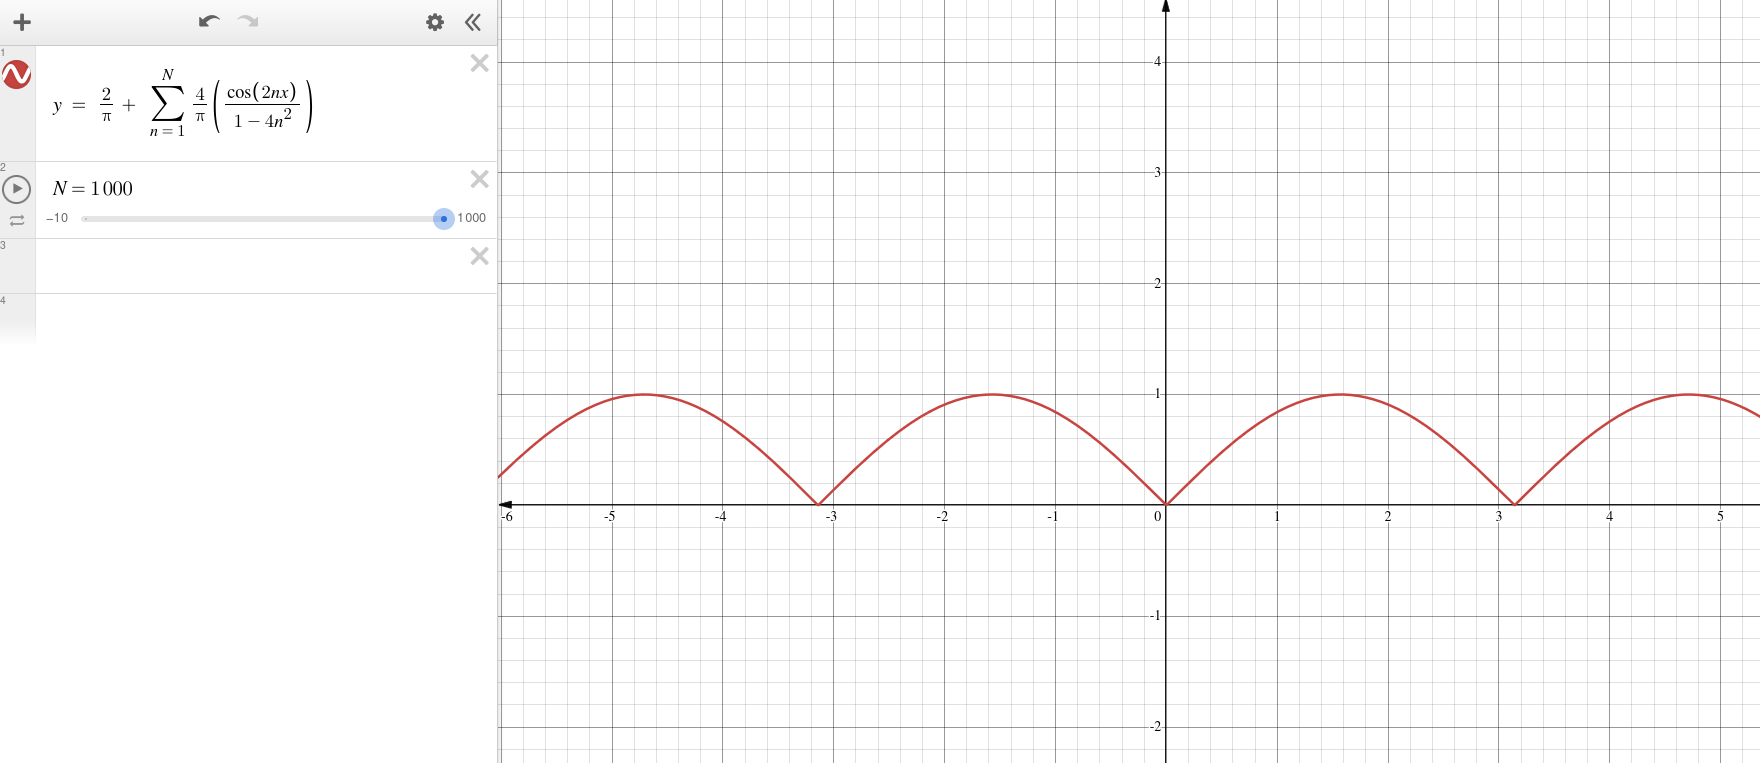
\includegraphics[width=0.7\textwidth]{photos/graf_onda_completa.png}
  \caption{Imagen de la se\~nal en su serie}
\end{figure}

Desarrollando los primeros terminos de la serie obtenemos los siguiente

\[x(t) = \dfrac{2}{\pi} - \dfrac{4}{3\pi} cos(2t) - \dfrac{4}{15\pi} cos(4t) - \dfrac{4}{35\pi} cos(6t)\]

\begin{figure}[H]
  \centering
  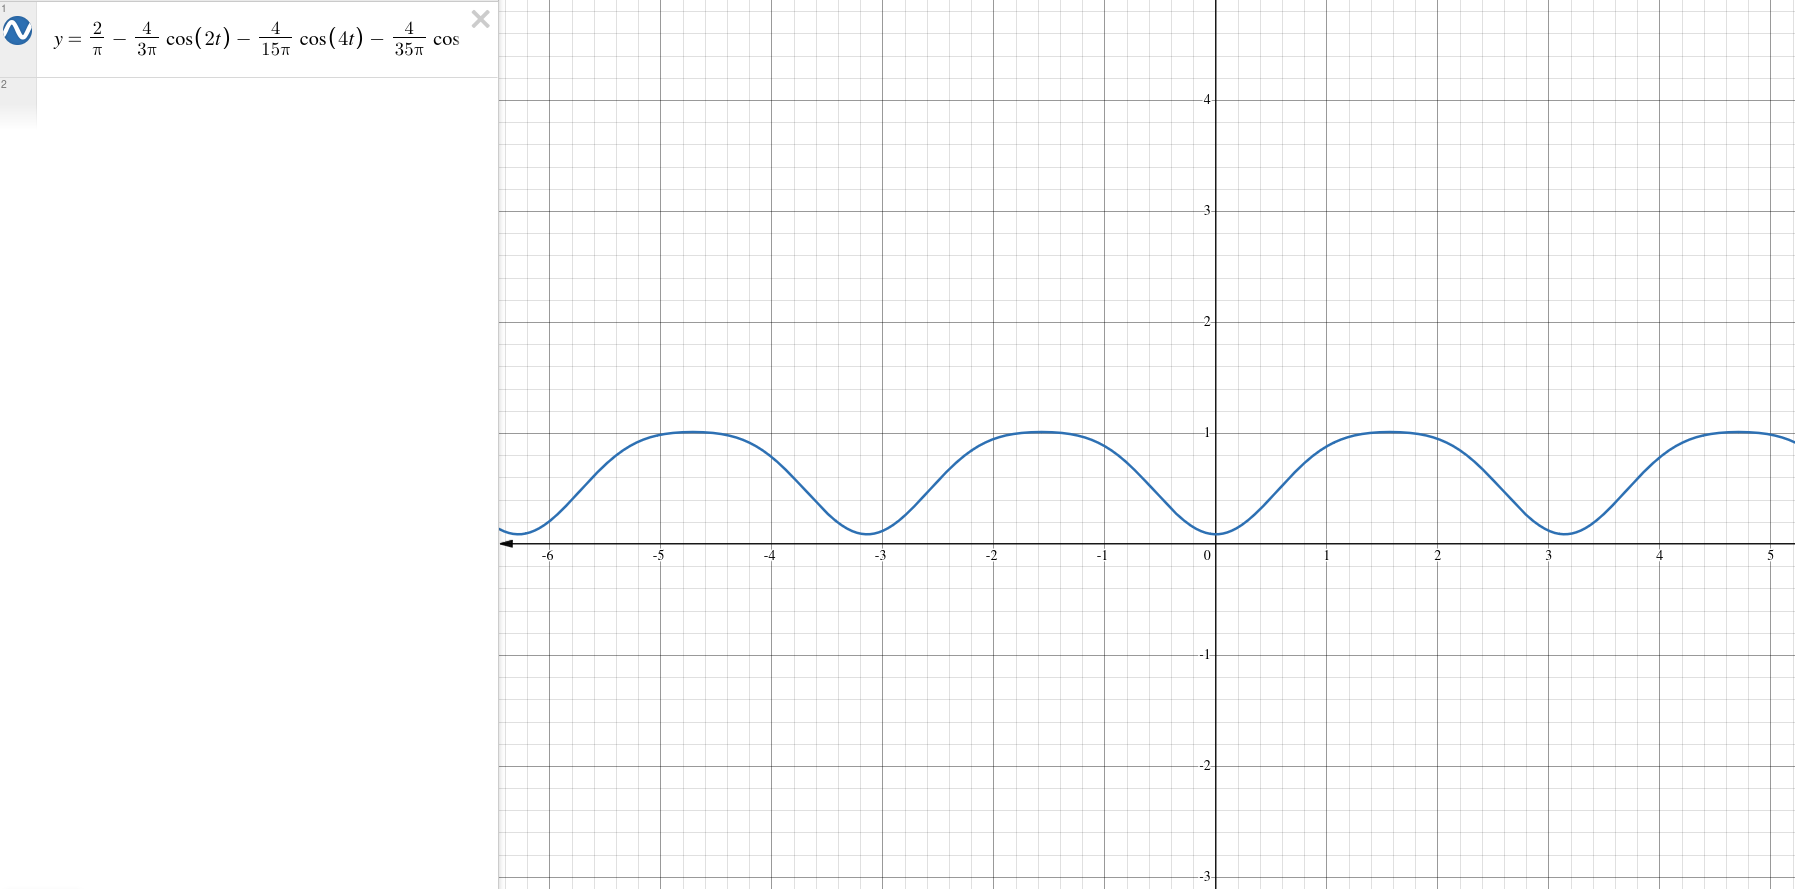
\includegraphics[width=0.7\textwidth]{photos/graf_aprox_onda_completa.png}
  \caption{Imagen de los primeros terminos de la serie}
\end{figure}

Para expresar la se\~nal en su segunda forma (la cual si es posible ya que la se\~nal con la que estamos trabajando SI es real) nos es de suma importancia saber si la se\~nal tiene simetr\'ia, par, impar o no tiene simetr\'ia.

Para que sea par debe cumplir con que $f(-t) = f(t)$

$$f(-t) = |sen(-t)| = |-sen(t)| = |sen(t)| = f(t) $$

Por lo que verificamos que la se\~nal es par, entonces

$$b_n = 0 $$

$$a_0 = \dfrac{1}{T} \int_{<T>} x(t) dt $$

$$a_0 = \dfrac{1}{\pi} -\cos (t) \bigg\rvert_{0}^{\pi} = -\dfrac{1}{\pi} (-1-1) = \dfrac{2}{\pi} $$

$$a_n = \dfrac{2}{T} \int_{<T>} x(t) \cos \bigg(\dfrac{2n\pi t}{T} \bigg) $$

$$a_n = \dfrac{2}{\pi} \int_{0}^{\pi} sen(t) cos(2nt) dt $$

Anteriormente se realizo el calculo, con la diferencia de tener un 2 en el numerador

$$a_n = \dfrac{4}{\pi(1-4n^2)} $$

\[x(t) = \dfrac{2}{\pi} + \sum_{n=1}^{\infty} \dfrac{4}{\pi(1-4n^2) cos(2nt)} \]

Llegando al mismo resultado obtenido anteriomente. Ahora procederemos a calcular la potencia media de la se\~nal mediante el teorema de Parseval.

\[P_m = \dfrac{1}{T} \int_{<T>} f(t)^2 dt = \sum_{n=-\infty}^{\infty} |C_n|^2 \]

Lo calcularemos mediante ambos procedimientos y luego verificaremos la semejanza entre ambas alternativas

$$P_m = \dfrac{1}{\pi} \int_{0}^{\pi} sen^2 (t) dt $$

$$P_m = \dfrac{1}{\pi} \int_{0}^{\pi} \dfrac{1-cos(2t)}{2} dt$$

$$P_m = \dfrac{1}{\pi} \int_{0}^{\pi} \dfrac{1}{2} dt - \int_{0}^{\pi} cos(2t) dt $$

$$P_m = \dfrac{1}{\pi} \dfrac{\pi}{2} = \dfrac{1}{2} $$

\[P_m = |C_0|^2 + 2 \sum_{n=1}^{\infty} |C_n|^2 \]

$$|C_0|^2 = \dfrac{4}{\pi^2} $$

$$|C_n|^2 = \dfrac{4}{\pi^2(1-4n^2)^2} $$

\[P_m = \dfrac{4}{\pi^2} \bigg[1 + 2\sum_{n=1}^{\infty} \dfrac{1}{(1-4n^2)^2} \bigg] \]

Desarrollando 4 terminos de la serie

\[P_m = \dfrac{4}{\pi^2} \bigg[1 + 2 \bigg(\dfrac{1}{9} + \dfrac{1}{225} + \dfrac{1}{1225} + \dfrac{1}{3969} \bigg) \bigg] \]

$$P_m = 0,499816 $$

Verificando que el valor obtenido por ambas alternativas es el mismo, con una aproximacion mediante la serie del $99,962\percent$

\subsection{Se\~nal sinusoidal rectificada de media onda}

\begin{figure}[H]
  \centering
  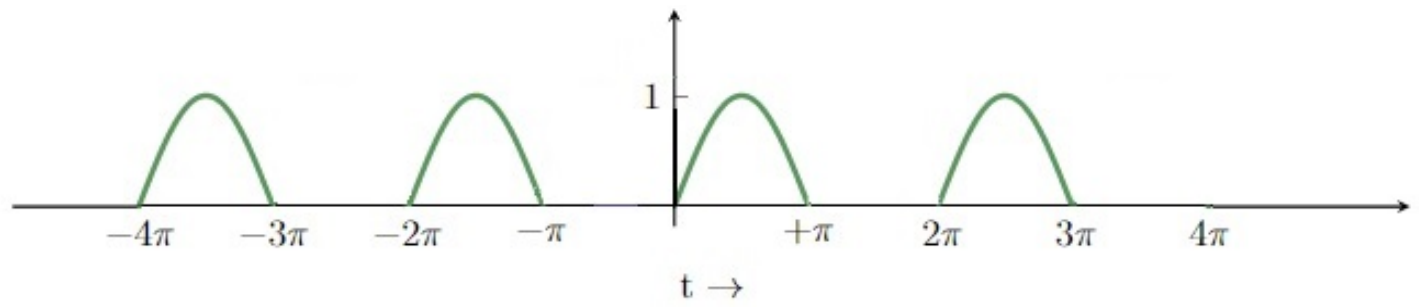
\includegraphics[width=0.8\textwidth]{photos/onda_media.png}
\end{figure}

$$C_n = \dfrac{1}{T} \int_{0}^{T} x(t) e^{-jn\omega_0t} dt$$

$$C_n = \dfrac{1}{2\pi} \int_{0}^{\pi} sen(t) e^{-jn\omega t} dt + \int_{\pi}^{2\pi} sen(t) e^{-jn\omega t} dt $$

En el gr\'afico de la funci\'on se puede observar que solamente existe entre los valores $0$ y $\pi$ en cambio entre $\pi$ y $2\pi$ vale 0, por ende integrarlo vale 0.

$$C_n = \dfrac{1}{2\pi} \int_{0}^{\pi} \bigg(\dfrac{e^{jt} - e^{-jt}}{2j} \bigg) e^{-jnt} dt $$

$$C_n = \dfrac{1}{j4\pi} \bigg[\int_{0}^{\pi} e^{jt(1-n)} dt - \int_{0}^{\pi} e^{-jt(1+n)} dt \bigg] $$

$$C_n = \dfrac{1}{j4\pi} \bigg[\dfrac{e^{jt(1-n)}}{j(1-n)} \bigg\rvert_{0}^{\pi} - \dfrac{e^{-jt(1+n)}}{-j(1+n)} \bigg\rvert_{0}^{\pi} \bigg] $$

$$C_n = \dfrac{1}{j4\pi} \bigg[\dfrac{1}{j} \dfrac{e^{j\pi(1-n)}-1}{(1-n)} + \dfrac{e^{-j\pi(1+n)}-1}{(1+n  )} \bigg] $$

$$e^{j\pi(1-n)} = e^{j\pi} e^{-jn\pi} = -(-1)^n $$

$$e^{-j\pi(1+n)} = e^{-j\pi} e^{-jn\pi} = -(-1)^n $$

$$C_n = -\dfrac{1}{4\pi} \bigg[\dfrac{-((-1)^n + 1)}{1-n} + \dfrac{-((-1)^n + 1)}{1+n} \bigg] $$

$$C_n = \dfrac{(-1)^n + 1}{4\pi} \bigg(\dfrac{1}{1-n} + \dfrac{1}{1+n} \bigg) $$

$$\dfrac{1}{1-n} + \dfrac{1}{1+n} = \dfrac{-2}{(n^2-1)} $$

$$C_n = -\dfrac{(-1)^n + 1}{2\pi(n^2-1)} $$

Para todo n impar $C_n = 0$ excepto en $\pm 1$, en $n=1$

$$C_1 = \dfrac{1}{2\pi} \int_{0}^{\pi} \bigg(\dfrac{e^{jt} - e^{-jt}}{2j} \bigg) e^{-jt} dt $$

$$C_1 = \dfrac{1}{j4\pi} \int_{0}^{\pi} \bigg(1- e^{-2jt} \bigg) dt $$

$$C_1 = \dfrac{1}{j4\pi} \bigg[\pi + \dfrac{e^{-2j\pi} - 1}{2j} \bigg] $$

$$C_1 = -\dfrac{j}{4} $$

Para el caso de $n=-1$

$$C_{-1} = \dfrac{1}{2\pi} \int_{0}^{\pi} \bigg(\dfrac{e^{jt} - e^{-jt}}{2j} \bigg) e^{jt} dt $$

$$C_{-1} = \dfrac{1}{j4\pi} \int_{0}^{\pi} \bigg(e^{2jt} - 1 \bigg) dt$$

$$C_{-1} = \dfrac{1}{j4\pi} \bigg[\bigg(\dfrac{e^{2jt}}{2j} - t \bigg)\bigg\rvert_{0}^{\pi} \bigg]$$

$$C_{-1} = \bigg[\dfrac{e^{2jt}}{8\pi}\bigg\rvert_{0}^{\pi} \bigg] - \bigg[\dfrac{-t}{j4t}\bigg\rvert_{0}^{\pi} \bigg] $$

$$C_{-1} = 0 - \dfrac{1}{j4} $$

$$C_{-1} = \dfrac{j}{4} $$

$$x(t) = $$

Ahora para el c\'alculo de los coeficientess $a_n$ y $b_n$ simplemente debemos conocer la matriz de
cambio de base la cual es $a_0 = C_0$ , $a_n = 2Re(C_n)$ , $b_n = -2Im(C_n)$.

\[
a_0 = \frac{1}{\pi}
\]

\[
a_n =
\begin{cases}
0 & \forall \, n \text{ impar} \\
\dfrac{2}{\pi(1-n^2)} & \forall \, n \text{ par}
\end{cases}
\]

\[
b_n =
\begin{cases}
\dfrac{1}{2} & n = 1 \\
0 & \forall \, n > 1
\end{cases}
\]

Ahora podemos escribir a $x(t)$ desarrollando los primeros valores de la serie

$$x(t) = \dfrac{1}{\pi} + \dfrac{1}{2}sen(t) + \dfrac{2}{\pi} \bigg[-\dfrac{1}{3} cos(2t) - \dfrac{1}{15} cos(4t) - \dfrac{1}{35} cos(6t)\bigg] $$

Procederemos a calcular la potencia media

$$P_m = \dfrac{1}{T} \int_{<T>} x(t) dt $$

$$P_m = \dfrac{1}{2\pi} \int_{0}^{\pi} sen(t)^2 dt $$

$$P_m = \dfrac{1}{2\pi} \cdot \dfrac{\pi}{2} $$

$$P_m = \dfrac{1}{4}$$
